\section{Problem 3-3}
\label{sec:problem3}

Given $\vect{r}(t_0)$, $\ivect{v}(t_0)$ at $t_0 = 1329.16$ min for Case 1, the Kepler-equation solver of Problem 3-2 is used to find the eccentric anomaly $E$, true anomaly $\nu$, and the PCI position and inertial velocity $\vect{r}(t)$, $\ivect{v}(t)$ at $t = 3885.73$ min, with $\mu = 398600~\text{km}^3\cdot\text{s}^{-2}$. The result is compared against a direct numerical integration of the two-body ODE (\texttt{ode113}-equivalent, Problem 3-1) at $t_f$ and over a 100-subinterval time series spanning $[t_0, t_f]$.

\programoutput{outputs/problem3.txt}

\begin{figure}[H]
    \centering
    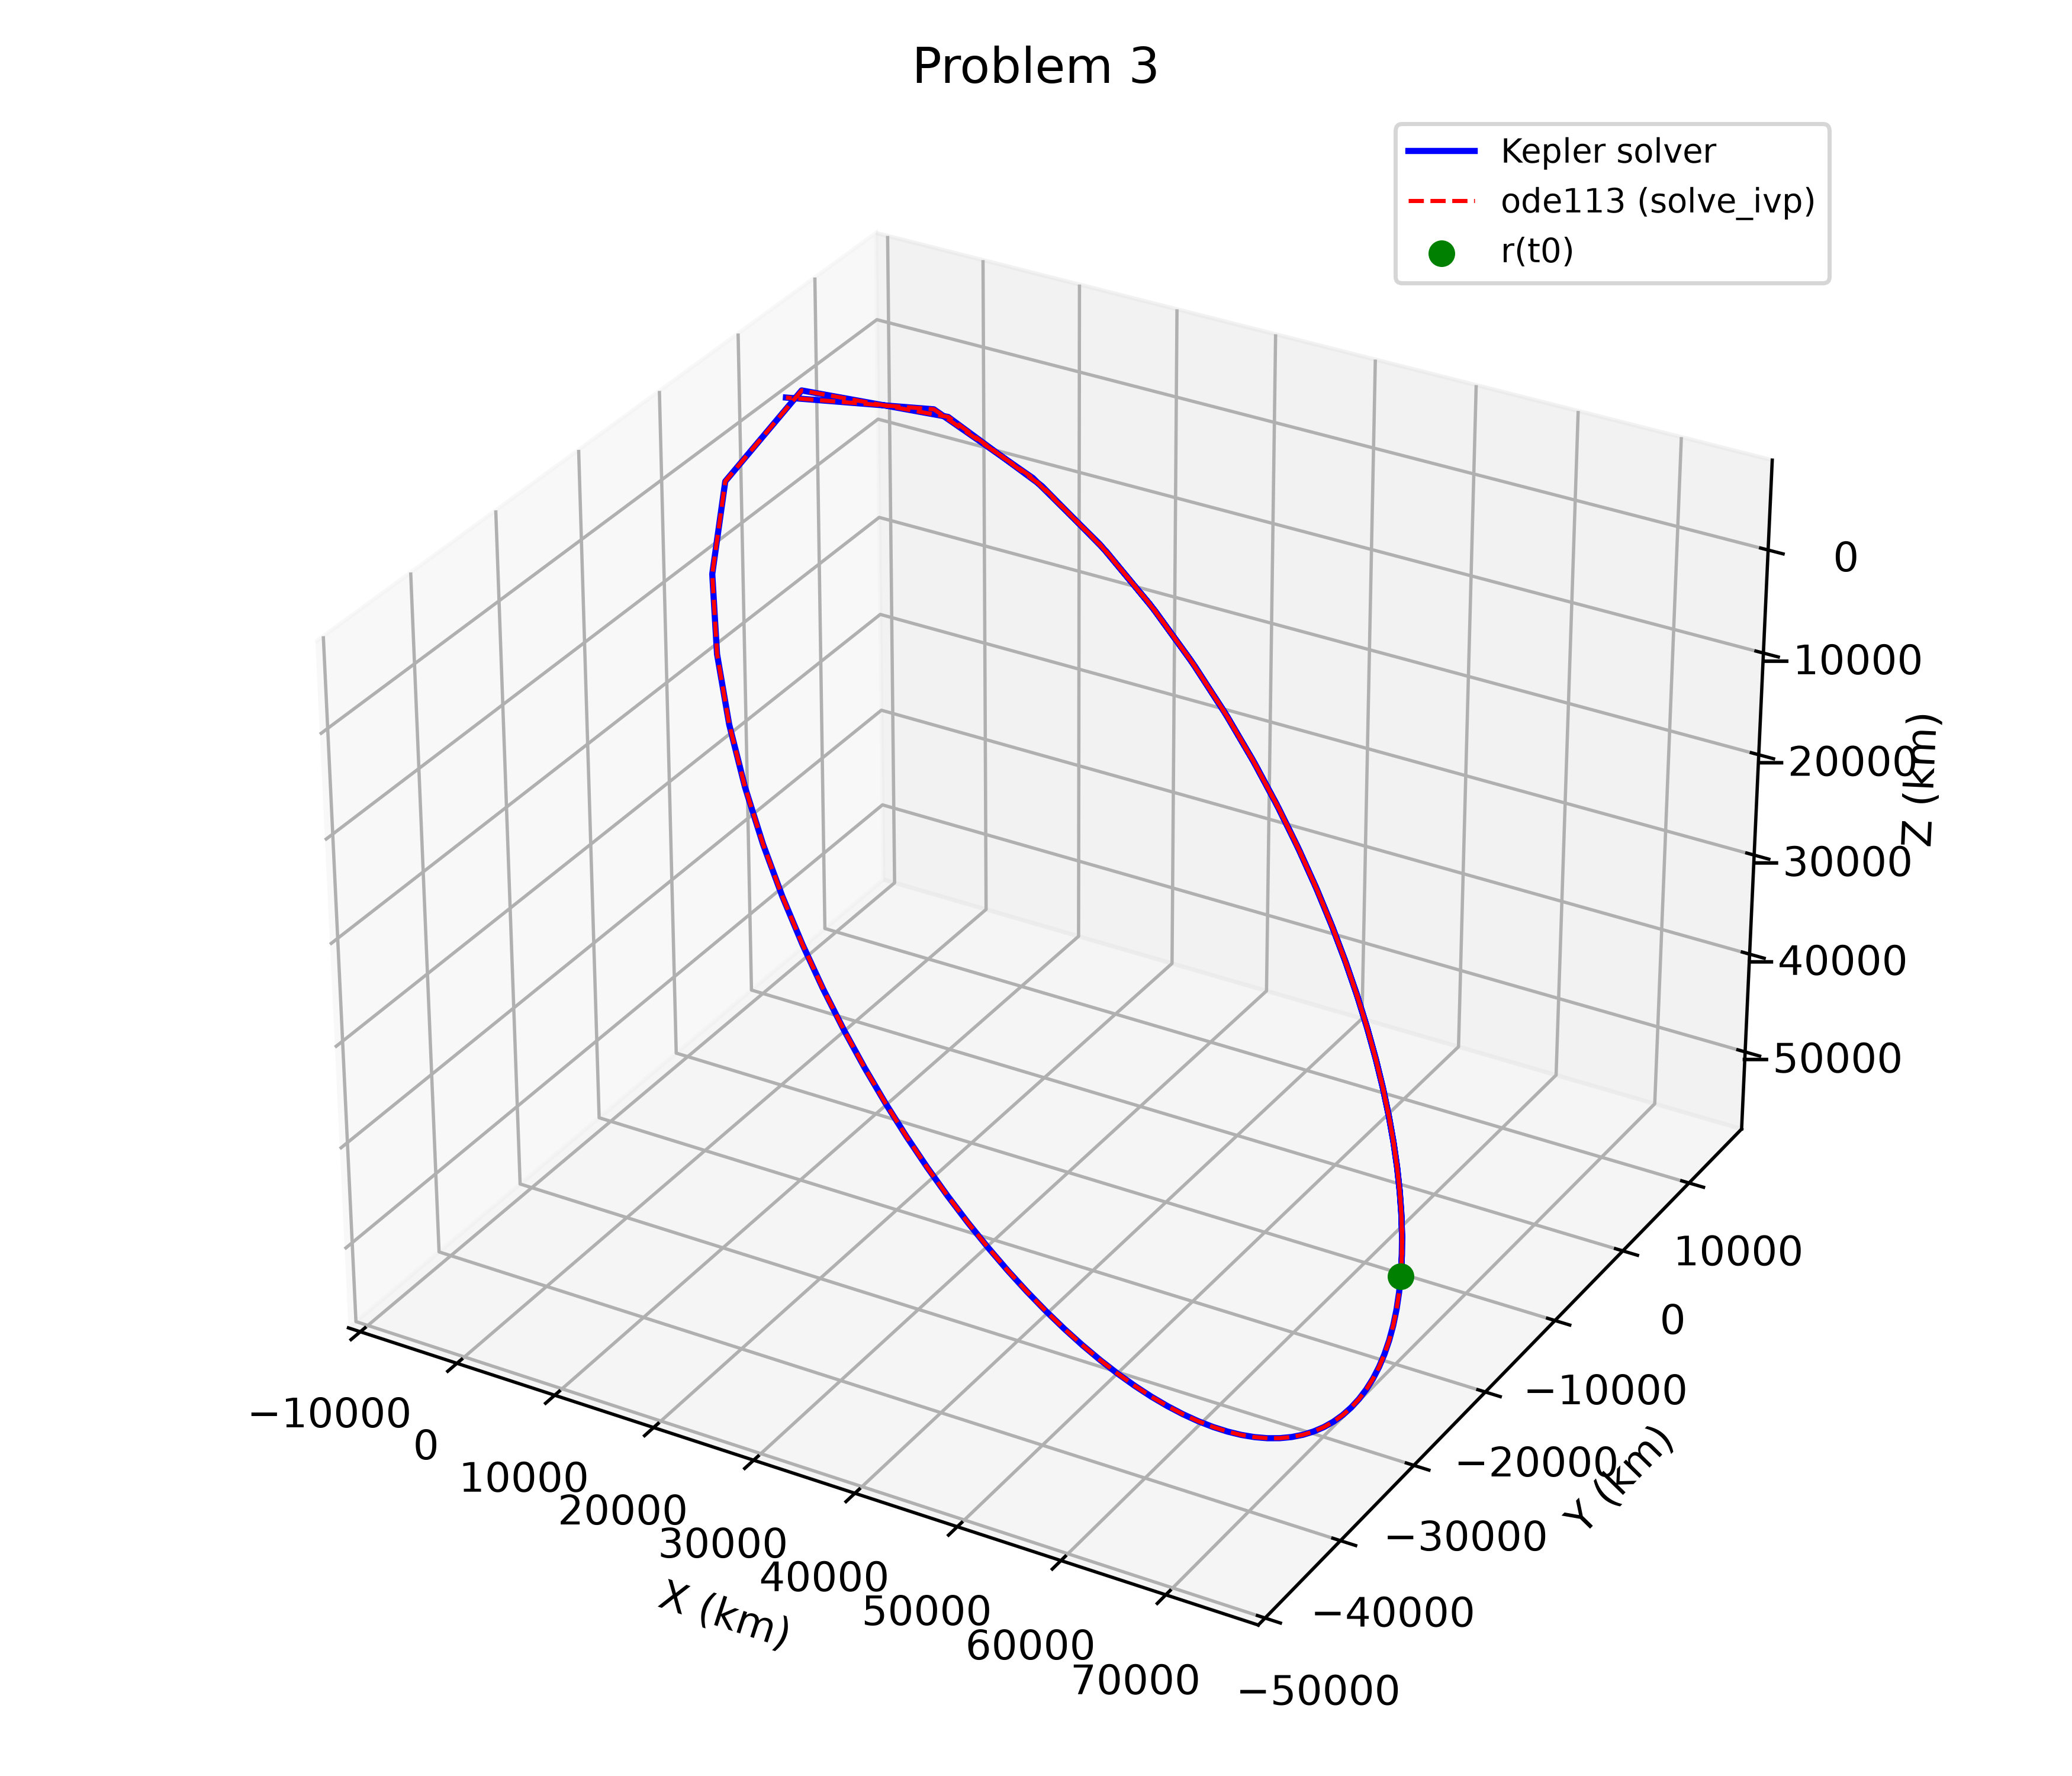
\includegraphics[width=0.75\textwidth]{figures/problem3_orbit.png}
    \caption{PCI position time series from the Kepler solver compared to \texttt{ode113}, Problem 3-3.}
\end{figure}

\FloatBarrier
